% 11-761 Language and Statistics
% Assignment 3 

\pdfoutput=1
\documentclass[11pt]{article}
\usepackage[left=1in,top=1in,right=1in,bottom=1in,nohead,nofoot]{geometry}
\usepackage{amsmath}
\usepackage{amsthm}
\usepackage{hyperref}
\usepackage{verbatim}
\usepackage{float}
\usepackage{graphicx}
\usepackage{longtable}
\usepackage{todonotes}
\newcommand{\f}[2]{\frac{#1}{#2}}
\newcommand{\ngram}{\mbox{$n$-gram}}

\newcommand{\leocomment}[1]{\todo[inline,color=red!40,caption={Leo's comment}]{#1}} 
\newcommand{\hectcomment}[1]{\todo[inline,color=green!40,caption={Hector's comment}]{#1}} 
\newcommand{\dicomment}[1]{\todo[inline,color=violet!40,caption={Hector's comment}]{#1}} 
\newcommand{\zhoucomment}[1]{\todo[inline,color=blue!40,caption={Hector's comment}]{#1}} 

\restylefloat{table}
\restylefloat{figure}

\begin{document}

\title{11-761 Language and Statistics - Spring 2013\\
Course Project}
\author{Leonid Boytsov, Zhou You, Di Wang, Hector Liu}
\date{}
\maketitle

\thispagestyle{empty}
\setlength{\parindent}{0pt}

\begin{abstract}
Our experiments indicate that 
an \ngram-based approach to synthetic documents outperforms other methods.
It allows us to achieve the accuracy 0.9 using the provided training set and the
slightly higher accuracy 0.91, if we train our model on the larger training data
(created by our group).
By using the 3-gram and 4-gram models alone, one can get accuracy as high as 0.88.
In the case of the soft metric, additional data allows us to improve the average
likelihood by a larger margin, namely, from 0.78 to 0.89.
We use a generative approach and train different models (the soft-margin SVM and 
the L1-regularized logistic regression)
to produce class labels and likelihoods.
\end{abstract}

\begin{figure}[H]\centering
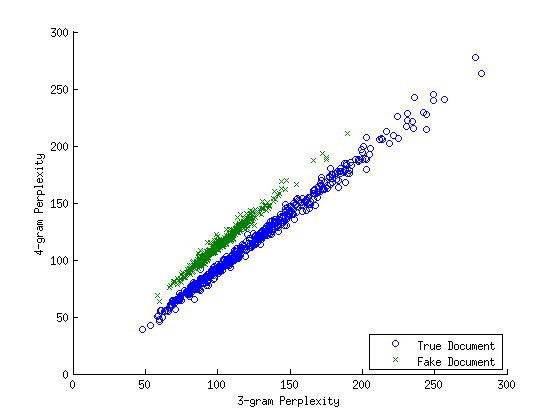
\includegraphics[scale=0.7]{erroranalysisGram34.png}
\caption{Perplexities for 3- and 4-gram models.\label{Fig1}}
\end{figure}


\end{document}
